\section{Introduction}
\label{section:introduction}

Over the last several years, we have witnessed a number of advances in mobile
computing technology. Mobile devices are now available in a variety of form
factors, such as glasses, watches, smartphones, tablets, personal robots, and
even cars. These devices come equipped with powerful processors, ample storage,
and a diverse array of sensors. Coupled with advances in operating systems and
middleware for mobile devices, programmers can now avail rich programming APIs
to build software (``\textit{apps}'') that leverage these advances in hardware.
Modern app markets contain hundreds of thousands of apps, and the number and
diversity of apps available to end-users has further contributed to the
popularity of mobile devices. These advances in hardware and software have made
mobile devices viable replacements for desktop computers.

At the same time, we are also witnessing a fundamental shift in the practice of
software development due largely to the dynamics of mobile app development.
Until a few years ago, the task of developing software (targeting mainly
desktop computers) was mostly confined to teams of software engineers, either
in the open-source community or at IT companies. In contrast, it is common even
for individuals or small teams to build and distribute software via mobile app
markets. Such teams, or individuals, may lack the expertise and experience of a
large team of developers and often face economic and time constraints during
app development.  Nevertheless, mobile app development teams aim to maximize
revenue by making their apps available on a wide variety of mobile devices,
\ie~those running software stacks such as Android, iOS, and Windows. Apps that
are available for a wide variety of mobile devices can reach a large user base,
and can therefore generate more revenue either through app purchases or via
in-app advertisements.

One way to build apps for different mobile platforms is to create customized
versions of apps for each platform, \eg~a separate version of the app for
Android, iOS and Windows devices. However, this approach leads to multiple
versions of the app's code-base, which are difficult to maintain and evolve
over time. Moreover, this approach is poorly-suited for small mobile app
development teams, which must now dedicate resources to create, maintain and
evolve different versions of the app for each mobile platform.

As a result of these shortcomings, developers are increasingly adopting
\textit{cross-platform mobile app development frameworks}. These frameworks
allow developers to program the app's logic once in a high-level language, and
provide tool-support to allow the app to execute on a number of mobile
platforms. 

\begin{figure*}[t!]
\centering
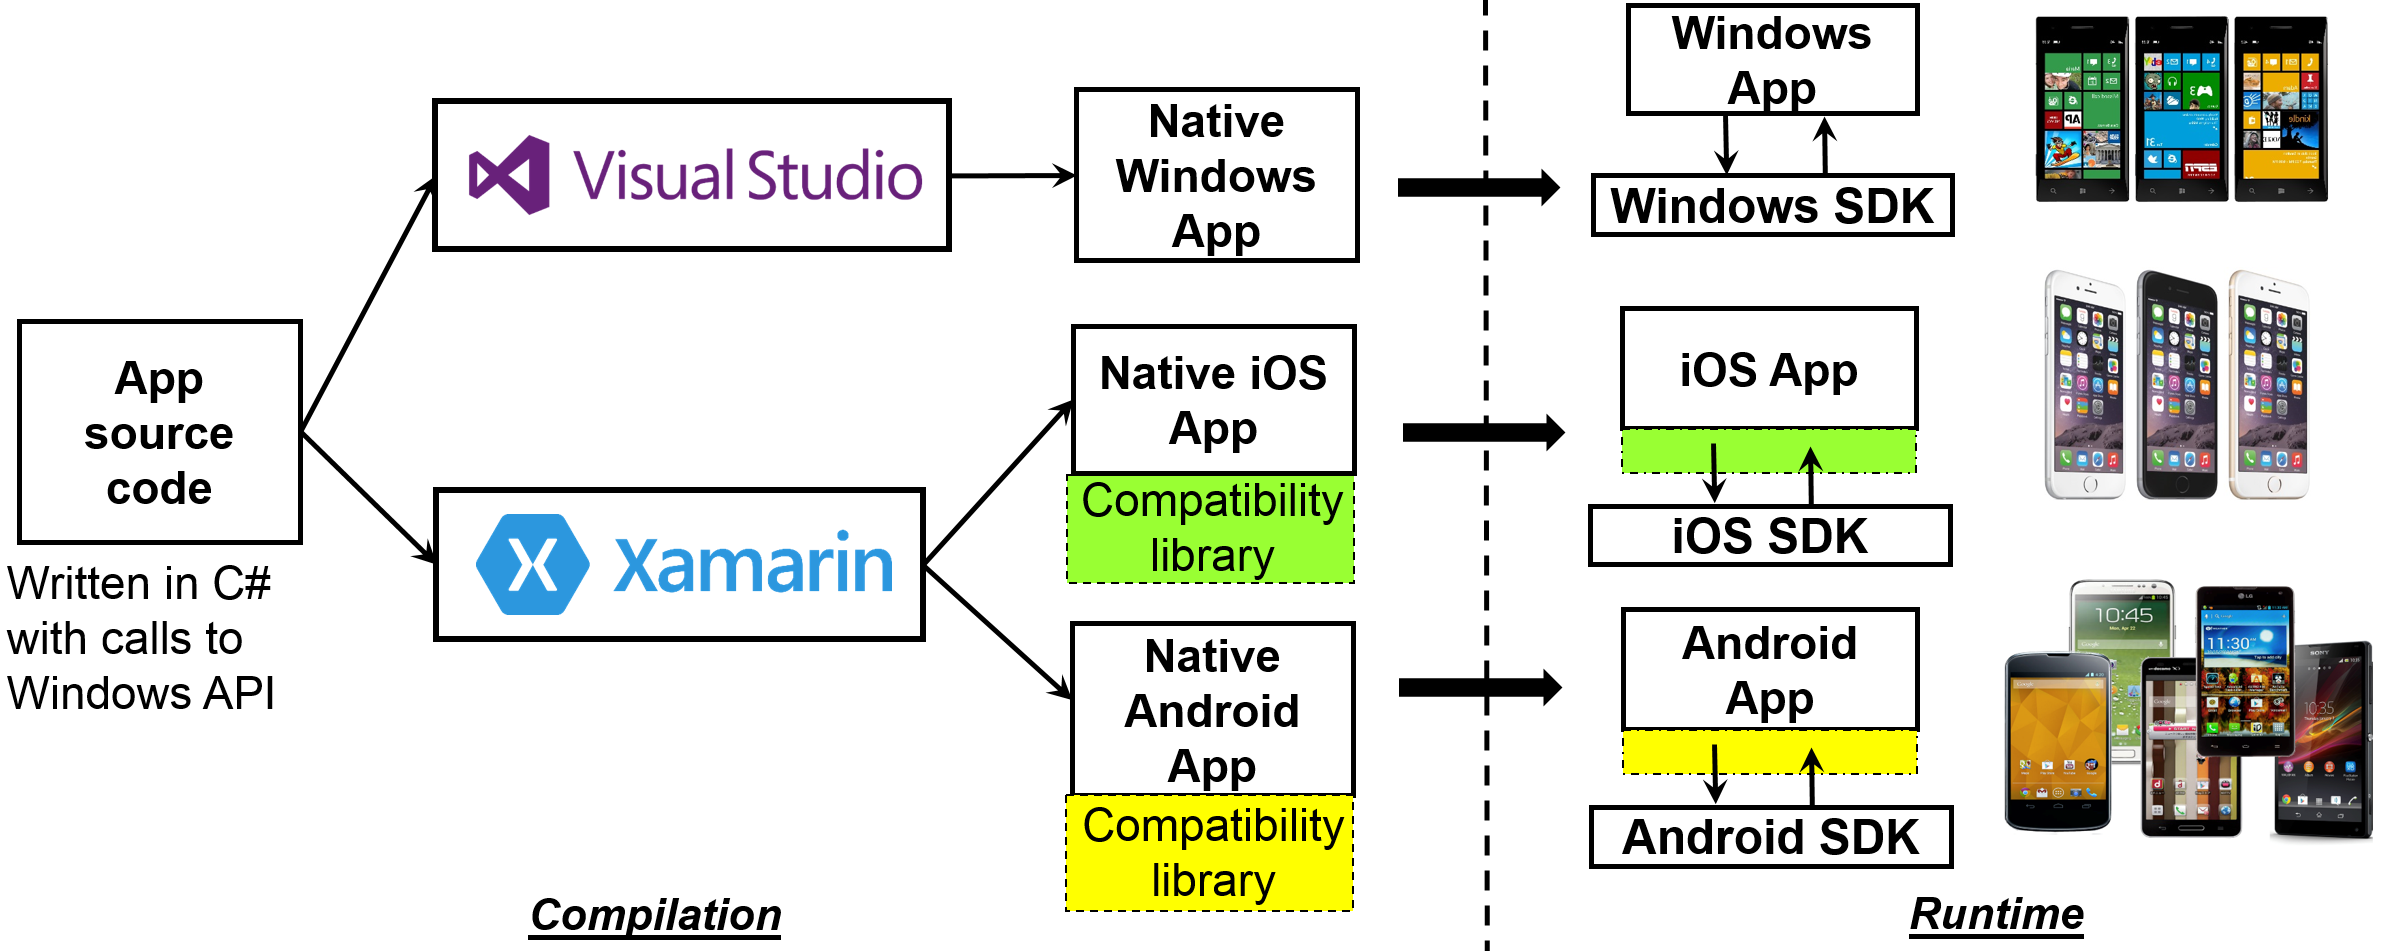
\includegraphics[keepaspectratio=true,width=0.9\textwidth]{figures/xptools-overview.png}
\mycaption{Overall operation of a cross-platform mobile app development
framework, using Xamarin as a concrete example. Developers build apps as they
would for the Windows Phone, in C\# using calls to the API of the Windows Phone
SDK. This code can directly be compiled to Windows Phone apps using the Visual
Studio toolchain. Xamarin allows developers to use the same source code to
build native Android or iOS apps. Xamarin provides compatibility libraries
that translate Windows SDK API calls in the code to the relevant API calls of
the underlying Android and iOS SDKs.}{\label{figure:xplatform-overview}}
\end{figure*}

There are two broad classes of cross-platform frameworks available today.  The
first class, which we call \textit{Web-based frameworks}, allows developers to
build mobile apps using languages popularly used to build Web applications,
such as HTML5, JavaScript, and CSS. Examples of such frameworks include Adobe
PhoneGap~\cite{phonegap}, Sencha~\cite{sencha} and IBM
MobileFirst~\cite{worklight}.  Developers specify the app's logic and user
interface using one or more of the Web-development languages.  However, these
languages do not contain primitives to allow apps to access resources on the
phone, \eg~peripherals such as the camera and microphone, the address book, and
phone settings. Thus, Web-based frameworks provide supporting runtime libraries
that end-users must download and execute on their mobile devices. Mobile apps
interface with these libraries to access resources on the mobile devices---such
mobile apps are also popularly called hybrid mobile apps.  Web-based frameworks
allow developers to rapidly prototype mobile apps.  However, these frameworks
are ill-suited for high-performance apps, such as games or those that use
animation. The expressiveness of the resulting mobile apps is also limited by
the interface exported by the runtime libraries offered by the frameworks.


The second class, which we call \textit{native frameworks}, addresses the above
challenges. Examples of such frameworks include Xamarin~\cite{xamarin},
Apportable~\cite{apportable} and MD$^2$~\cite{md2:sac13,myappconverter}. These
frameworks generally support a \textit{home platform} and one or more
\textit{target platforms}. Developers build mobile apps as they normally would
for the home platform, and leverage the framework's support to automatically
produce apps for the target platforms as well. For example, the home platform
for Xamarin is Windows Phone, and developers build apps using C\# and the API
of the Windows Phone SDK. The Xamarin framework allows developers to
automatically build Android and iOS apps using this code base (see
\figref{figure:xplatform-overview}). Likewise, the home platform for Apportable
is iOS. Developers build apps using Objective-C and the iOS SDK, and leverage
Apportable to produce Android apps from this code base.  In this paper, we will
focus on native frameworks for cross-platform mobile app development. 

When an app developer uses native frameworks, he implicitly expects the apps to
behave consistently across the home and target platforms. Realizing this
expectation depends to a large extent on the fidelity with which the native
framework translates the API calls to SDK of the home platform to the
corresponding SDK of the target platform(s). Unfortunately, this translation is
a complex task because the platform must correctly encode the semantics of both
the home platform and target platform SDK and the relationship between them.
This complexity translates into bugs in the frameworks, \eg~as of mid-December
2014, Xamarin's Bugzilla database shows a history of about 17,600 bug reports,
5,100 of which are still unresolved (listed as ``open'' or ``new''), while
Apportable's bug database shows a history of 820 bug reports, 449 of which are
unresolved.

In this paper, we develop an approach to test native cross-platform app
development tools. Specifically, we aim to discover cases where the behavior of
the application on the home platform is inconsistent with the behavior of its
counterpart on a target platform. Our approach is based on \textit{differential
testing}~\cite{mckeeman:difftest:1998}. We generate random test cases (using
methods described in prior work~\cite{randoop:icse07}), which in our case are
mobile apps in the source language of the home platform. We then use this code
to produce two versions of the app, one for the home platform, and one for the
target platform using the native framework. We then execute the apps and
examine the resulting state for inconsistent behavior.  When two versions of
the app are produced from the same source code, any differences in the behavior
across the versions are indicative of a problem either in the home platform's
SDK, the target platform's SDK, or the way the native framework translates
between the two SDKs.

To realize this approach, we must address two issues::
%
\begin{mylist}
%
\item \textbf{How can we generate effective test cases?} The key research
challenge here is that the space of valid programs that we can generate as test
cases is essentially unbounded. While we could sample from this space, the
effectiveness of these test cases in inducing inconsistent behavior is
questionable.

To address this challenge, we observe that the main difficulty in building
cross-platform mobile app development tools is \textit{translating between the
semantics of the SDKs of the home and target platforms}. Our test-case
generator therefore produces programs that contain random sequences of
invocations to the home platform's SDK. We then observe whether the resulting
apps on the home and target platforms behave consistently. By focusing on the
SDK alone, our approach narrows testing to the most error-prone components of
the cross-platform frameworks.

\item \textbf{How can we check for inconsistent behavior?} Each of our test
cases is compiled into a full-fledged app, one each for the home and target
platforms. When we run the corresponding apps, we must observe their behaviors
to identify inconsistencies. The main research challenge here is in defining a
suitable notion of ``behavior.''

We address this challenge by observing all data structures that are reachable
from the variables defined in the test cases. We serialize these data
structures into a standard format, and compare the serialized versions on the
home and target platforms. Assuming that the state of the home and target
platforms is the same before the test cases are executed, the final state in
each platform after the test cases have been executed must also be the same.
If not, we consider this inconsistent behavior and report an error.
%
\end{mylist}

We have prototyped this approach in a tool called \tool, which we have applied
to test the Xamarin framework using Android as the target platform. Using
\tool, we have found \checkme{47} inconsistencies, which corresponded to bugs
either in Xamarin or the Microsoft SDK (we have reported many of these to
Xamarin or Microsoft). To date, one of these bugs has also been fixed in the
development branch of Xamarin.
